\ifdefined\iscombined
	\lecturetitle{An Example in Mechanical System Analysis}
\else
\documentclass{article}
\usepackage{xparse}
\usepackage{changepage}
\usepackage{listings}
\usepackage{amsthm}
\usepackage{comment}
\usepackage{amsmath}
\usepackage{braket}
\usepackage{amsfonts}
\usepackage{sectsty}
\usepackage{hyperref}
\usepackage{fancyhdr}
\usepackage[top=1in,bottom=1in,left=1in,right=1in]{geometry}
\usepackage{float}
\usepackage{graphicx}
\usepackage{mathtools}
\usepackage{tikz}
\usetikzlibrary{arrows,calc,patterns,decorations.pathmorphing,decorations.markings}
\usepackage{circuitikz}

\date{
	\vspace{-.75em}
	{\large \today}
}

\title{
	\vspace*{-1.5em}
	{\Huge Lecture 10} \\
	\vspace{-1em}
	\rule{\textwidth/4}{.01em} \\
	\vspace{-.25em}
	{\Large An Example in Mechanical System Analysis}
	\vspace{-.75em}
}

\author{
	{\large Matthew Farah}
}

\hypersetup{
	colorlinks=true,
	linkcolor=blue,
	filecolor=magenta,
	urlcolor=blue,
	citecolor=blue,
	anchorcolor=blue
}

\fancyhead{}
\fancyhead[L]{\today}
\fancyhead[R]{Lecture 10 - An Example in Mechanical System Analysis}

\setlength{\parindent}{0cm}

\newcounter{example}
\renewcommand{\theexample}{\arabic{example}}

\newenvironment{example}[1][]{
	\refstepcounter{example}
	\begin{adjustwidth}{1.5em}{}
	\noindent\textbf{\ifx&#1&Example \theexample:\else Example \theexample \ (#1):\fi}
	\ignorespaces
}{
	\vspace{.5em}
	\end{adjustwidth}
}

\newenvironment{solution}{
	\vspace{.5em}
	\par
	\begin{adjustwidth}{1.5em}{}
	\textbf{{Solution:}}
	\par
	\vspace{.5em}
}{
	\vspace{1em}
	\end{adjustwidth}
}

\newcounter{subexample}
\renewcommand{\thesubexample}{\alph{subexample}}

\newenvironment{subexample}{
	\setcounter{step}{0}
	\refstepcounter{subexample}
	\vspace{1em}\par\noindent
	\begin{adjustwidth}{1.5em}{}
	\noindent\textbf{(\thesubexample)}
	\ignorespaces
}{
	\par
	\vspace{1em}
	\end{adjustwidth}
}

\renewenvironment{proof}{
	\vspace{.5em}\par\noindent
	\begin{adjustwidth}{1.5em}{}
	\emph{Proof:}\par\vspace{1em}
	\setlength{\parindent}{0cm}
}{
	\end{adjustwidth}
}

\newtheorem{theorem}{Theorem}

\renewenvironment{theorem}[1][]{
	\refstepcounter{theorem}
	\vspace{1em}\par\noindent
	\begin{adjustwidth}{1.5em}{}
	\noindent\textbf{\ifx&#1&Theorem \thetheorem:\else Theorem \thetheorem \ (#1):\fi}
	\ignorespaces
}{
	\vspace{.5em}
	\end{adjustwidth}
}

\newtheorem{lemma}{Lemma}

\renewenvironment{lemma}[1][]{
	\refstepcounter{lemma}
	\vspace{1em}\par\noindent
	\begin{adjustwidth}{1.5em}{}
	\noindent\textbf{\ifx&#1&Lemma \thelemma:\else Lemma \thelemma \ (#1):\fi}
	\ignorespaces
}{
	\vspace{.5em}
	\end{adjustwidth}
}

\makeatother
\makeatletter

\newcounter{step}
\renewcommand{\thestep}{\Roman{step}}

\newenvironment{step}{
	\refstepcounter{step}
	\vspace{1em}\par\noindent
	\ignorespaces\noindent\textbf{(\thestep)}
	\ignorespaces
}{
	\par
	\vspace{1em}
}

\sectionfont{\fontsize{12}{12}\bfseries}
\subsectionfont{\fontsize{10}{12}\normalfont}
\subsubsectionfont{\fontsize{10}{12}\normalfont}

\begin{document}

\maketitle
\pagestyle{fancy}

\fi

\begin{itemize}
	\item \textbf{Midterm hints:}
	\begin{itemize}
		\item There will be four questions on the midterm:
		\begin{enumerate}
			\item One on Laplace transforms.
			\item One on circuits.
			\item One on mechanical systems.
			\item One on either:
			\begin{itemize}
				\item Block diagram reductions.
				\item A Rotational systems.
			\end{itemize}
		\end{enumerate}
	\end{itemize}

	\item Generally, the degrees of freedom of a mechanical system equals the number of masses/inertias in it.
	\begin{itemize}
		\item Note: this is not always the case.
	\end{itemize}
\end{itemize}

\begin{example}
	Find the transfer function for the third body, $G(s) = \frac{X_3(s)}{F(s)}$, given the system:

	\vspace{1em}

	\begin{figure}[H]
		\centering
		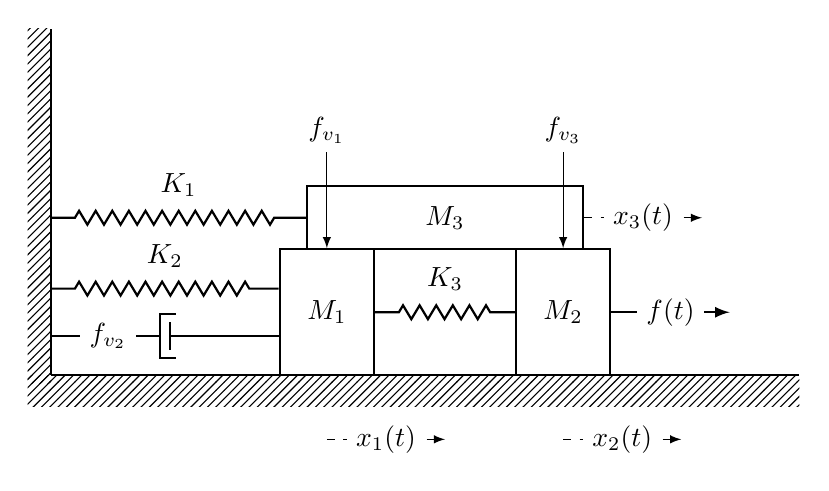
\begin{tikzpicture}[>=latex]
			\tikzstyle{spring}=[thick,decorate,decoration={zigzag,pre length=0.3cm,post length=0.3cm,segment length=6}]
			\tikzstyle{damper}=[thick,decoration={markings,
				mark connection node=dmp,
				mark=at position 0.5 with
				{
					\node (dmp) [thick,inner sep=0pt,transform shape,rotate=-90,minimum width=15pt,minimum height=3pt,draw=none] {};
					\draw [thick] ($(dmp.north east)+(2pt,0)$) -- (dmp.south east) -- (dmp.south west) -- ($(dmp.north west)+(2pt,0)$);
					\draw [thick] ($(dmp.north)+(0,-5pt)$) -- ($(dmp.north)+(0,5pt)$);
				}
			}, decorate]

			\fill [pattern=north east lines] (0.2,-0.9) rectangle (0.5,3.6);
			\fill [pattern=north east lines] (0.2,-0.8) rectangle (10, -1.2);
			\draw [thick] (0.5,-0.8) -- (0.5,3.6);
			\draw [thick] (0.5,-0.8) -- (10,-0.8);

			\node (M1) [draw, thick, minimum width=1.2cm, minimum height=1.6cm] at (4,0) {$M_1$};
			\node (M2) [draw, thick, minimum width=1.2cm, minimum height=1.6cm] at (7,0) {$M_2$};
			\node (M3) [draw, thick, minimum width=3.5cm, minimum height=0.8cm] at (5.5,1.2) {$M_3$};

			\draw [spring] (0.5,1.2) -- (M3.west) node[midway, above=4pt, fill=white] {$K_1$};
			\draw [spring] (0.5,0.3) -- ($(M1.west) + (0,0.3)$) node[midway, above=4pt, fill=white] {$K_2$};
			\draw [damper] (0.5,-0.3) -- ($(M1.west) + (0,-0.3)$) node[near start, fill=white] {$f_{v_2}$};
			\draw [spring] (M1.east) -- (M2.west) node[midway, above=4pt, fill=white] {$K_3$};

			\draw [->, thin] ($(M1.north) + (0,1.5)$) -- (M1.north) node[at start, fill=white] {$f_{v_1}$};
			\draw [->, thin] ($(M2.north) + (0, 1.5)$) -- (M2.north) node[at start, fill=white] {$f_{v_3}$};

			\draw [->, thick] (M2.east) -- ++(1.5,0) node[midway, fill=white] {$f(t)$};

			\draw [dashed, ->] ($(M1.south) + (0,-0.8)$) -- ++(1.5,0) node[midway, fill=white] {$x_1(t)$};
			\draw [dashed, ->] ($(M2.south) + (0,-0.8)$) -- ++(1.5,0) node[midway, fill=white] {$x_2(t)$};
			\draw [dashed, ->] ($(M3.east)$) -- ++(1.5,0) node[midway, fill=white] {$x_3(t)$};
		\end{tikzpicture}
	\end{figure}

	\vspace{1em}

	And that:

	\begin{alignat*}{3}
		M_1 &= 4\,\text{kg}, \quad &&M_2 = 5\,\text{kg}, \quad &&M_3 = 5\,\text{kg} \\
		f_{v_1} &= 2\,\text{Ns/m}, \quad &&f_{v_2} = 2\,\text{Ns/m}, \quad &&f_{v_3} = 3\,\text{Ns/m} \\
		K_1 &= 5\,\text{N/m}, \quad &&K_2 = 4\,\text{N/m}, \quad &&K_3 = 4\,\text{N/m},
	\end{alignat*}

	\begin{align*}
		\det\left( \begin{bmatrix} 4s^2 + 4s + 8 & -4 & -2s \\\\ -4 & 5s^2 + 3s + 4 & -3s \\\\ -2s & -3s & 5s^2 + 5s + 5 \end{bmatrix} \right) &= 100s^6 + 260s^5 + 544s^4 + 652s^3 + 484s^2 + 280s + 80
	\end{align*}
\end{example}

\begin{solution}
	To solve this problem, we will need to do the following:

	\begin{enumerate}
		\item Find the forces acting on $M_1$ by displacing it by $x_1(t)$ and holding all the other masses still in the Laplace domain.
		\item Use the superposition principle to include the forces acting on $M_1$ by $M_2$ and $M_3$ in the Laplace domain.
		\item Create an equation for $M_1$ representing all the forces acting on it.
		\item Repeat steps 1) to 3) for $M_2$ and $M_3$.
		\item Put all equations into matrix form.
		\item Solve for $X_3(s)$ using Cramer's rule.
	\end{enumerate}

	\begin{step}
		Find the forces acting on $M_1$ by moving it and all other masses still in the Laplace domain.
	\end{step}

	Looking at the diagram, moving $M_1$ by some displacement $x_1(t)$ in the direction indicated, $M_1$ experiences the following forces:

	\begin{enumerate}
		\item The force resisting motion due to $M_1$'s mass (represented by $s^2 M_1 X_1(s)$ in the Laplace domain).
		\item The force of friction with $M_3$ $(f_{v_1} s X_1(s))$.
		\item The force of the viscous damper $(f_{v_2} s X_1(s))$.
		\item The force of the spring with spring constant $K_2$ $(K_2 X_1(s))$.
		\item The force of the spring with spring constant $K_3$ $(K_3 X_1(s))$.
	\end{enumerate}

	In free body diagram (FBD) form, this looks like:

	\vspace{1em}

	\begin{figure}[H]
		\centering
		\begin{tikzpicture}[>=latex']
			\draw (0,-1.4) rectangle (1.5,2.8);
			\node at (0.75,0.7) {$M_1$};
			\draw[->] (0,1.8) -- node[midway, fill = white]{$M_1 s^2X_1(s)$} (-3.2,1.8);
			\draw[->] (0,0.7) -- node[midway, fill = white]{$K_2 X_1(s)$} (-3.2,0.7);
			\draw[->] (0,-0.6) -- node[midway, fill = white]{$f_{v_2} s X_1(s)$} (-3.2,-0.6);
			\draw[->] (4.7,1.8) -- node[midway, fill = white]{$f_{v_1} s X_1(s)$} (1.5,1.8);
			\draw[->] (4.7,-0.6)  -- node[midway,below]{$K_3 X_1(s)$} (1.5,-0.6);
			\draw[dashed, ->] (0.75,3.3) -- node[midway, fill = white]{$X_1(s)$} (2.75,3.3);
		\end{tikzpicture}
	\end{figure}

	\vspace{1em}

	\begin{step}
		Include the forces acting on $M_1$ by moving $M_2$ and $M_3$ in the Laplace domain.
	\end{step}

	By inspection and use of Newton's second law of motion, we can see that displacing $M_2$ and $M_3$ by $X_2(s)$ and $X_3(s)$ respectively, we obtain the following FBD of $M_1$:

	\vspace{1em}

	\begin{figure}[H]
		\centering
		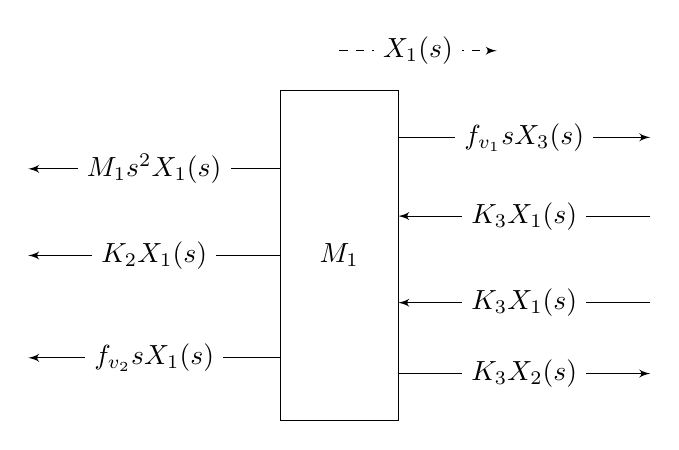
\begin{tikzpicture}[>=latex']
			\draw (0,-1.4) rectangle (1.5,2.8);
			\node at (0.75,0.7) {$M_1$};
			\draw[->] (0,1.8) -- node[midway, fill = white]{$M_1 s^2 X_1(s)$} (-3.2,1.8);
			\draw[->] (0,0.7) -- node[midway, fill = white]{$K_2 X_1(s)$} (-3.2,0.7);
			\draw[->] (0,-0.6) -- node[midway, fill = white]{$f_{v_2} s X_1(s)$} (-3.2,-0.6);
			\draw[->] (1.5, 2.2) -- node[midway, fill = white]{$f_{v_1} s X_3(s)$} (4.7,2.2);
			\draw[->] (4.7,1.2) -- node[midway, fill = white]{$K_3 X_1(s)$} (1.5, 1.2);
			\draw[->] (4.7, 0.1) -- node[midway, fill = white]{$K_3 X_1(s)$} (1.5, 0.1);
			\draw[->] (1.5, -0.8) -- node[midway, fill = white]{$K_3 X_2(s)$} (4.7, -0.8);
			\draw[dashed, ->] (0.75,3.3) -- node[midway, fill = white]{$X_1(s)$} (2.75,3.3);
		\end{tikzpicture}
	\end{figure}

	\vspace{1em}

	\begin{step}
		Express all forces acting on $M_1$ as an equation.
	\end{step}

	Now, we know all net forces on an object must equal 0 (forces acting to the right equals forces acting to the left). So:

	\begin{equation*}
		\begin{array}{lrl}
			& M_1 s^2 X_1(s) + K_2 X_1(s) + f_{v_1} s X_1(s) + f_{v_2} s X_1(s) + K_3 X_1(s) =& K_2 X_2(s) + f_{v_1} s X_3(s) \\
			\implies & (M_1 s^2 + K_2 + f_{v_1} s + f_{v_2} s + K_3) X_1(s) =& K_2 X_2(s) + f_{v_1} s X_3(s) \\
			\implies & (M_1 s^2 + K_2 + K_3 + (f_{v_1} + f_{v_2}) s) X_1(s) - K_2 X_2(s) - (f_{v_1} s) X_3(s) =& 0
		\end{array}
	\end{equation*} \\

	And by substituting for the values given, we arrive at our first equation:

	\begin{equation*}
		\begin{array}{lrl}
			& (4s^2 + 4 + 4 + (2 + 2)s) X_1(s) - 4 X_2(s) - 2s X_3(s) =& 0 \\
			\implies & (4s^2 + 4s + 8) X_1(s) - 4 X_2(s) - 2s X_3(s) =& 0 \quad \ldots (1)
		\end{array}
	\end{equation*} \\

	\begin{step}
		Do the same for $M_2$ and $M_3$.
	\end{step}

	As before, examining the diagram gives the following FBDs for $M_2$ and $M_3$ (holding all other masses still):

	\vspace{1em}

	\begin{figure}[H]
		\centering
		\begin{tikzpicture}[>=latex']
			\draw (0,-1.4) rectangle (1.5,2.8);
			\node at (0.75,0.7) {$M_2$};
			\draw[->] (0,1.8) -- node[midway, fill = white]{$M_2 s^2 X_2(s)$} (-3.2,1.8);
			\draw[->] (0,0.7) -- node[midway, fill = white]{$f_{v_3} sX_2(s)$} (-3.2,0.7);
			\draw[->] (0,-0.6) -- node[midway, fill = white]{$K_3 X_2(s)$} (-3.2,-0.6);
			\draw[->] (1.5,0.7) -- node[midway, fill = white]{$F(s)$} (4.7,0.7);
			\draw[dashed, ->] (0.75,3.3) -- node[midway, fill = white]{$X_2(s)$} (2.75,3.3);
		\end{tikzpicture}
		\hspace{1em}
		\begin{tikzpicture}[>=latex']
			\draw (0,-1.4) rectangle (1.5,2.8);
			\node at (0.75,0.7) {$M_3$};
			\draw[->] (0,1.8) -- node[midway, fill = white]{$M_3 s^2 X_3(s)$} (-3.2,1.8);
			\draw[->] (0,-0.6) -- node[midway, fill = white]{$K_1 X_3(s)$} (-3.2,-0.6);
			\draw[->] (4.7,1.8) -- node[midway, fill = white]{$f_{v_1} sX_3(s)$} (1.5,1.8);
			\draw[->] (1.5,-0.6) -- node[midway, fill = white]{$f_{v_3} sX_3(s)$} (4.7,-0.6);
			\draw[dashed, ->] (0.75,3.3) -- node[midway, fill = white]{$X_3(s)$} (2.75,3.3);
		\end{tikzpicture}
	\end{figure}

	\vspace{1em}

	And by including the forces on $M_2$ by moving $M_1$, $M_3$, and the forces on $M_3$ by moving $M_1$, $M_2$, we get:

	\vspace{1em}

	\begin{figure}[H]
		\centering
		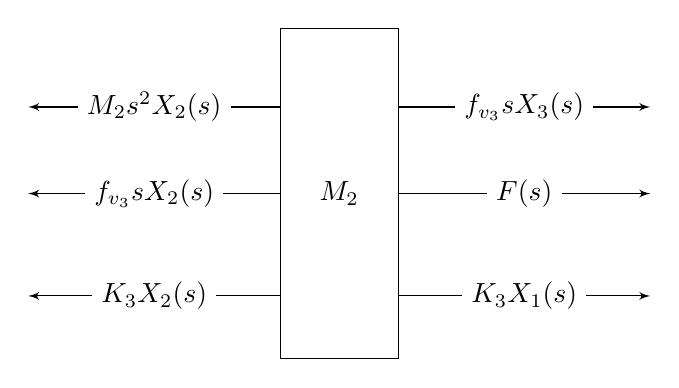
\begin{tikzpicture}[>=latex']
			\draw (0,-1.4) rectangle (1.5,2.8);
			\node at (0.75,0.7) {$M_2$};
			\draw[->] (0,1.8) -- node[midway, fill = white]{$M_2 s^2 X_2(s)$} (-3.2,1.8);
			\draw[->] (0,0.7) -- node[midway, fill = white]{$f_{v_3} s X_2(s)$} (-3.2,0.7);
			\draw[->] (0,-0.6) -- node[midway, fill = white]{$K_3 X_2(s)$} (-3.2,-0.6);
			\draw[->] (1.5,1.8) -- node[midway, fill = white]{$f_{v_3} s X_3(s)$} (4.7, 1.8);
			\draw[->] (1.5,0.7) -- node[midway, fill = white]{$F(s)$} (4.7,0.7);
			\draw[->] (1.5,-0.6) -- node[midway, fill = white]{$K_3 X_1(s)$} (4.7,-0.6);
		\end{tikzpicture}
		\hspace{1em}
		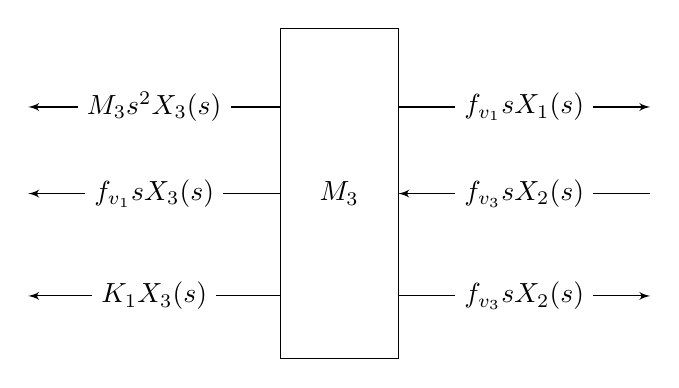
\begin{tikzpicture}[>=latex']
			\draw (0,-1.4) rectangle (1.5,2.8);
			\node at (0.75,0.7) {$M_3$};
			\draw[->] (0,1.8) -- node[midway, fill = white]{$M_3 s^2 X_3(s)$} (-3.2,1.8);
			\draw[->] (0,0.7) -- node[midway, fill = white]{$f_{v_1} s X_3(s)$} (-3.2,0.7);
			\draw[->] (0,-0.6) -- node[midway, fill = white]{$K_1 X_3(s)$} (-3.2,-0.6);
			\draw[->] (1.5,1.8) -- node[midway, fill = white]{$f_{v_1} s X_1(s)$} (4.7,1.8);
			\draw[->] (4.7,0.7) -- node[midway, fill = white]{$f_{v_3} s X_2(s)$} (1.5,0.7);
			\draw[->] (1.5,-0.6) -- node[midway, fill = white]{$f_{v_3} s X_2(s)$} (4.7,-0.6);
		\end{tikzpicture}
	\end{figure}

	\vspace{1em}

	We can express both FBDs in equation form as follows. For $M_2$:

	\begin{equation*}
		\begin{array}{lrl}
			& M_2 s^2 X_2(s) + f_{v_3} s X_2(s) + K_3 X_2(s) =& f_{v_3} s X_3(s) + F(s) + K_3 X_1(s) \\
			\implies & (M_2 s^2 + f_{v_3} s + K_2) X_2(s) =& f_{v_3} s X_3(s) + F(s) + K_3 X_1(s) \\
			\implies & -K_3 X_1(s) + (M_2 s^2 + f_{v_2} s + K_2) X_2(s) - f_{v_3} s X_3(s) =& F(s)
		\end{array}
	\end{equation*} \\

	And for $M_3$:

	\begin{equation*}
		\begin{array}{lrl}
			& M_3 s^2 X_3(s) + f_{v_1} s X_3(s) + f_{v_3} s X_3(s) + K_1 X_3(s) =& f_{v_1} s X_1(s) + f_{v_2} s X_2(s) \\
			\implies & (M_3 s^2 + \left(f_{v_1} + f_{v_3}\right) s + K_1) X_3(s) =& f_{v_1} s X_1(s) + f_{v_2} s X_2(s) \\
			\implies & -f_{v_1} s X_1(s) - f_{v_2} s X_2(s) + (M_3 s^2 + \left(f_{v_1} + f_{v_3}\right) s + K_1) X_3(s) =& 0
		\end{array}
	\end{equation*} \\

	And by substituting for the values we're given, we obtain the last two equations we need:

	\begin{align*}
		-4 X_1(s) + (5s^2 + 3s + 4) X_2(s) - 3s X_3(s) &= F(s) \quad \ldots (2) \\
		-2s X_1(s) - 3s X_2(s) + (5s^2 + 5s + 5) X_3(s) &= 0 \quad \ldots (3)
	\end{align*}

	\begin{step}
		Express equations in matrix form.
	\end{step}

	Putting equations $(1)$, $(2)$, and $(3)$ in matrix form, we have that:

	\begin{align*}
		\begin{bmatrix} 4s^2 + 4s + 8 & -4 & -2s \\\\ -4 & 5s^2 + 3s + 4 & -3s \\\\ -2s & -3s & 5s^2 + 5s + 5 \end{bmatrix} \begin{bmatrix} X_1(s) \\\\ X_2(s) \\\\ X_3(s) \end{bmatrix} &= \begin{bmatrix} 0 \\\\ F(s) \\\\ 0 \end{bmatrix}
	\end{align*}

	\begin{step}
		Solve for $X_3(s)$ using Cramer's rule.
	\end{step}

	Cramer's rule tells us that:

	\begin{align*}
		X_3(s) &= \frac{\det(A_3)}{\det(A)}
	\end{align*}

	Where:

	\begin{align*}
		A &= \begin{bmatrix} 4s^2 + 4s + 8 & -4 & -2s \\\\ -4 & 5s^2 + 3s + 4 & -3s \\\\ -2s & -3s & 5s^2 + 5s + 5 \end{bmatrix} \quad \text{(the matrix multiplying $\begin{bmatrix} X_1(s) \\\\ X_2(s) \\\\ X_3(s) \end{bmatrix}$)}
	\end{align*}

	And:

	\begin{align*}
		A_3 &= \begin{bmatrix} 4s^2 + 4s + 8 & -4 & 0 \\\\ -4 & 5s^2 + 3s + 4 & F(s) \\\\ -2s & -3s & 0 \end{bmatrix} \quad \text{(the result of swapping the third column of $A$ with $\begin{bmatrix} 0 \\\\ F(s) \\\\ 0 \end{bmatrix}$)}
	\end{align*}

	It's given in the question that:

	\begin{align*}
		\det(A) &= 100s^6 + 260s^5 + 544s^4 + 652s^3 + 484s^2 + 280s + 80
	\end{align*}

	So, we need only find $\det(A_3)$, which, by expanding along the third column for ease of calculation, is given by:

	\begin{align*}
		\det(A_3) &= (-1)^{3+1}(0)\left( (-4)(-3s) - (5s^2 + 3s + 4)(-2s) \right) \\
			& \quad + (-1)^{3+2} F(s) \left( (4s^2 + 4s + 8)(-3s) - (-4)(-2s) \right) \\
			& \quad + (-1)^{3+3}(0) \left( (4s^2 + 4s + 8)(5s^2 + 3s + 4) - (-4)(-4) \right) \\
			&= -(12s^3 + 12s^2 + 32s) F(s)
	\end{align*}

	Therefore:

	\begin{align*}
		X_3 &= \frac{\det(A_3)}{\det(A)} = \frac{-(12s^3 + 12s^2 + 32s) F(s)}{100s^6 + 260s^5 + 544s^4 + 652s^3 + 484s^2 + 280s + 80}
	\end{align*}

	Thus, $G(s)$ is given by:

	\begin{align*}
		\frac{X_3(s)}{F(s)} &= \frac{-(12s^3 + 12s^2 + 32s) F(s)}{100s^6 + 260s^5 + 544s^4 + 652s^3 + 484s^2 + 280s + 80} \div F(s) \\
			&= \frac{-(12s^3 + 12s^2 + 32s)}{100s^6 + 260s^5 + 544s^4 + 652s^3 + 484s^2 + 280s + 80}
	\end{align*}
\end{solution}

\ifdefined\iscombined
	\newpage
\else
	\end{document}
\fi
